\documentclass[12pt,a4paper]{article}
\usepackage[utf8]{inputenc}
\usepackage[T1]{fontenc}
\usepackage{amsmath}
\usepackage{amsfonts}
\usepackage{amssymb}
\usepackage{lipsum}
\usepackage{textcomp}

\usepackage{makecell} % linebreak dans une cellule
\usepackage{multicol} % twocols localement
\usepackage{vwcol} % idem mais avec largeur variable
\usepackage{color, colortbl} % colorer les tableaux
\usepackage{enumitem} % utiliser des lettres pour énumérer
\usepackage{wrapfig} % insérer des images dans dutexte
\usepackage{dashundergaps} % transformer du texte en ________
\usepackage{MnSymbol,wasysym} % smileys
\usepackage{ifthen}
\usepackage{soul} % teste barré \st

% --- geometry ---
\usepackage{geometry}
\geometry{legalpaper, margin=2cm}
% ---

% --- xcolor ---
\usepackage{xcolor}
\definecolor{lightgray}{gray}{0.9}
% ---

% --- tcolorboxes ---
\usepackage[most]{tcolorbox}
\newtcolorbox{definition}[2][]{%
  attach boxed title to top left
               = {yshift=-8pt},
  colback      = white,
  colframe     = gray,
  fonttitle    = \bfseries,
  colbacktitle = gray,
  title        = #2,#1,
  enhanced,
}
% ---


\renewcommand{\baselinestretch}{1.15} % augmenter l'interligne

\dashundergapssetup{
	teacher-gap-format=underline,
	gap-widen
}



\author{Paul Clavier}
\title{Chapitre 4 - Nombres décimaux et comparaison de nombres}

\begin{document}

% --- Section & subsection renum ---
\renewcommand\thesection{\Roman{section}}
\renewcommand\thesubsection{\arabic{subsection}}
% ---

% --- Selection manuelle de la version ---
%\TeacherModeOn
% ---

% --- Selection automatique de la version ---
\ifdefined\isprof
	\TeacherModeOn
\fi

% ---



\begin{center}
	\fbox{\parbox{\dimexpr\linewidth-2\fboxsep-2\fboxrule\relax}{\centering\huge Chapitre 4 - Nombres décimaux et comparaison de nombres}}
\end{center}

\section{Comparaison et rangement}

\subsection{Comparaison de deux nombres décimaux}

\begin{definition}{Définition}
Comparer deux nombre, c'est trouver lequel est le plus grand (ou le plus petit) ouu dire s'ils sont égaux.
\end{definition}

\textbf{Remarque}: On utilise les symboles $>$ pour «plus grand que» et $<$ pour «plus petit que». 

\begin{definition}{Règle}
Pour comparer deux nombres décimaux écrits sous forme décimale:
\begin{itemize}
\item on compare les \gap*{parties entières}
\item si les \gap*{parties entières} sont égales, on compare les \gap*{chiffres des dixièmes}
\item si les \gap*{chiffres des dixièmes} sont égales, on compare les \gap*{chiffres des centièmes}
\item et ainsi de suite jusqu'à ce que les deux nombres aient des chiffres différents
\end{itemize}
\end{definition}

\textbf{Exemple}: Compare les nombres 81,357 et 81,36
\begin{itemize}
\item on compare les parties entières des deux nombres
\item elles sont égales donc on compare les chiffres des dixièmes
\item ils sont égaux donc on compare les chiffres des centièmes
\item 5 < 6 donc 81,3\textbf{5}7 < 81,3\textbf{6}
\end{itemize} 

\textbf{Remarque}: Si les parties entières  sont égales, on peut comparer les parties décimales.

$\displaystyle 81,357 = 81+\frac{357}{1000}$ et $\displaystyle 81,36 = 81+\frac{36}{100} = 81+\frac{360}{1000}$.

Or 360 \gap*{millièmes} est plus grand que 357 \gap*{millièmes} donc 81,\textbf{36} > 81,\textbf{257}
 
\subsection{Rangement de nombres}

\begin{definition}{Vocabulaire}
\begin{itemize}
\item Ordre croissant: du plus \gap*{petit} au plus \gap*{grand}
\item Ordre décroissant: du plus \gap*{grand} au plus \gap*{petit}
\end{itemize}
\end{definition}

\textbf{Exemple}: range les nombres 25,342 - 253,42 - 25,243 - 235,42 - 25,324 dans l'ordre croissant.

\gap*{$ 25,243 < 25,324 < 25,342 < 235,42 < 253,42 $}

\section{Repérage sur une demi-droite graduée}

\begin{definition}{Définition}
Sur une \textbf{droite graduée}, l'abscisse d'un point est le nombre qui permet de repérer la position de ce point sur la droite.
\end{definition}

\textbf{Exemple}: Quelles sont les abscisses des points A et B?

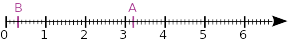
\includegraphics[scale=1]{img/abscisse-1.png} 

\begin{itemize}
\item Une unité est divisée en 10 parts égales, ce qui signifie d'elle est dévisée en 10 dixièmes
\item Le point A se trouve 2 dixièmes après 3 donc son abscisse est $3+\frac{2}{10}$, soit 3,2
\item Le point B se trouve 3 dixièmes après 0 donc son abscisse est $0+\frac{3}{10}$, soit 0,3
\end{itemize}

\begin{definition}{Notation}
On note A(3,1) et B(0,3)
\end{definition}













\end{document}